%----------------------------------------
\begin{frame}[fragile]
  \frametitle{First application}

{\Large\bf Using Temporal Constraints to Generate Tests}

\end{frame}

%----------------------------------------
\begin{frame}
  \frametitle{Command driven systems} \small

\begin{figure}
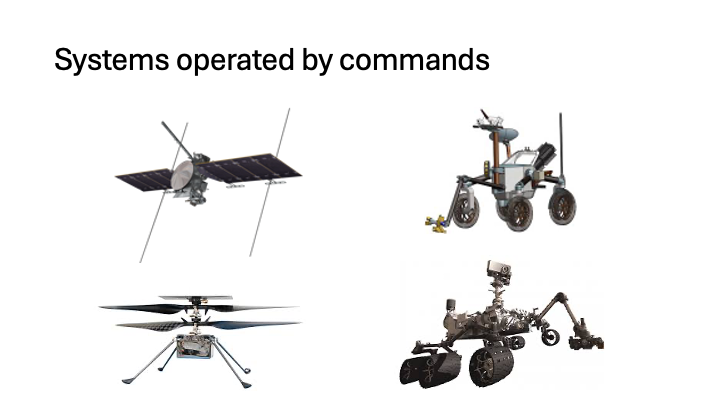
\includegraphics[width=1.0\textwidth]{figures/start1.png}
%\caption{Your caption}
\end{figure}

\begin{block}{}\scriptsize
The system is operated by commands being submitted to it.  
\end{block}

\end{frame}


%----------------------------------------
\begin{frame}
  \frametitle{Command driven system} \small

\begin{figure}
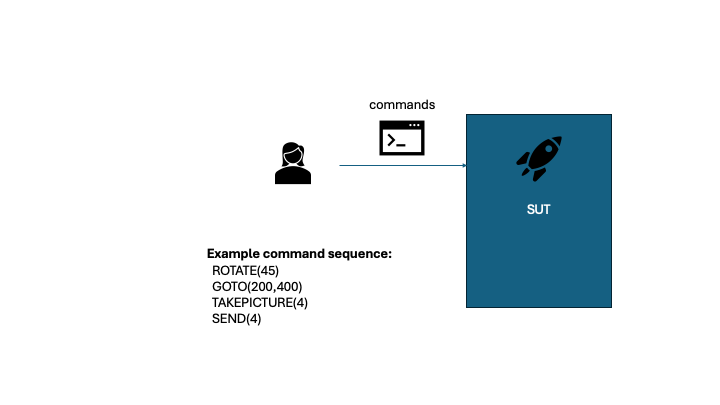
\includegraphics[width=1.0\textwidth]{figures/start2.png}
%\caption{Your caption}
\end{figure}

\begin{block}{}\scriptsize
Command driven systems of interest are those operated by sequences of commands.  
\end{block}

\end{frame}


%----------------------------------------
\begin{frame}
  \frametitle{Command driven system under test} \small

\begin{figure}
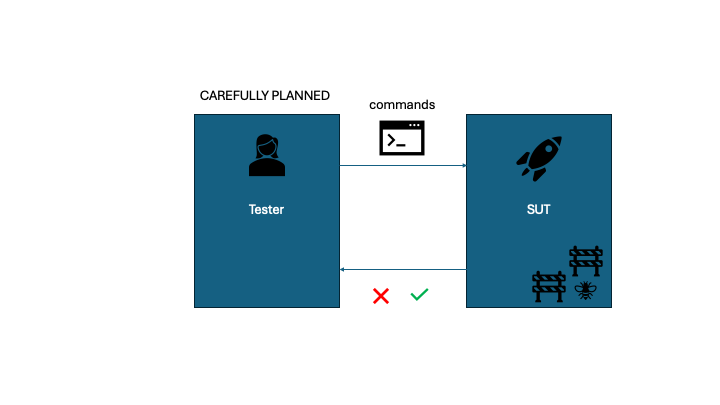
\includegraphics[width=1.0\textwidth]{figures/start3.png}
%\caption{Your caption}
\end{figure}

\begin{block}{}\scriptsize
Traditionally such a system is tested by manual creation of carefully planned command sequences.
\end{block}

\end{frame}


%----------------------------------------
\begin{frame}
  \frametitle{Command driven system under test} \small

\begin{figure}
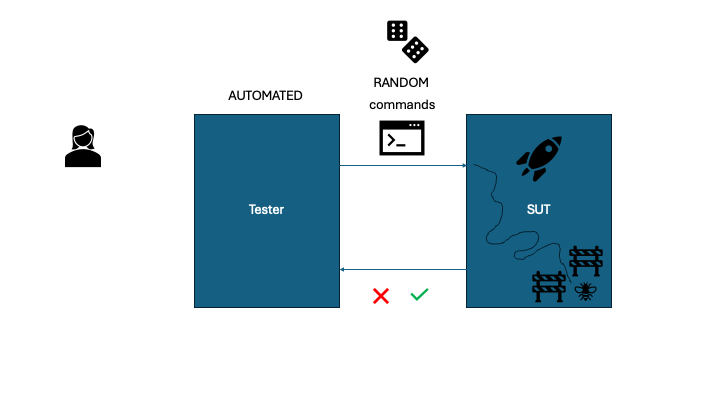
\includegraphics[width=1.0\textwidth]{figures/start4.png}
%\caption{Your caption}
\end{figure}

\begin{block}{}\scriptsize
However, this may not get into the corners of the SUT. We therefore want to fuzz test the SUT by sending random commands to it. But not too random, we want to constrain the randomness.
\end{block}

\end{frame}


%----------------------------------------
\begin{frame}
  \frametitle{Command driven system under test} \small

\begin{figure}
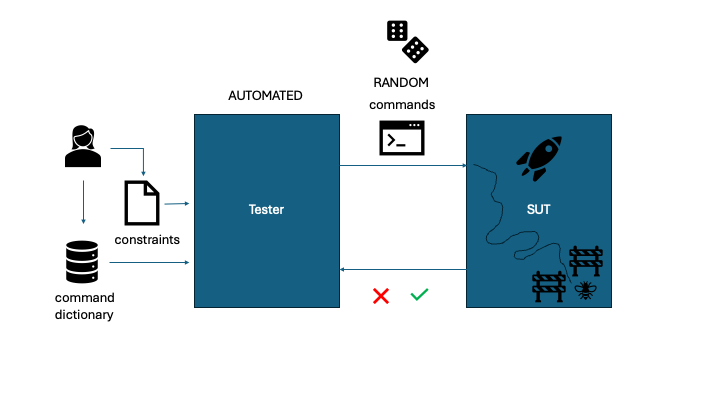
\includegraphics[width=1.0\textwidth]{figures/start5.png}
%\caption{Your caption}
\end{figure}

\begin{block}{}\scriptsize
The user defines what commands are possible and constraints on the randomness using an expressive
temporal logic.
\end{block}

\end{frame}


%----------------------------------------
\begin{frame}<0>
  \frametitle{Plan as a T-diagram} \small

\begin{figure}
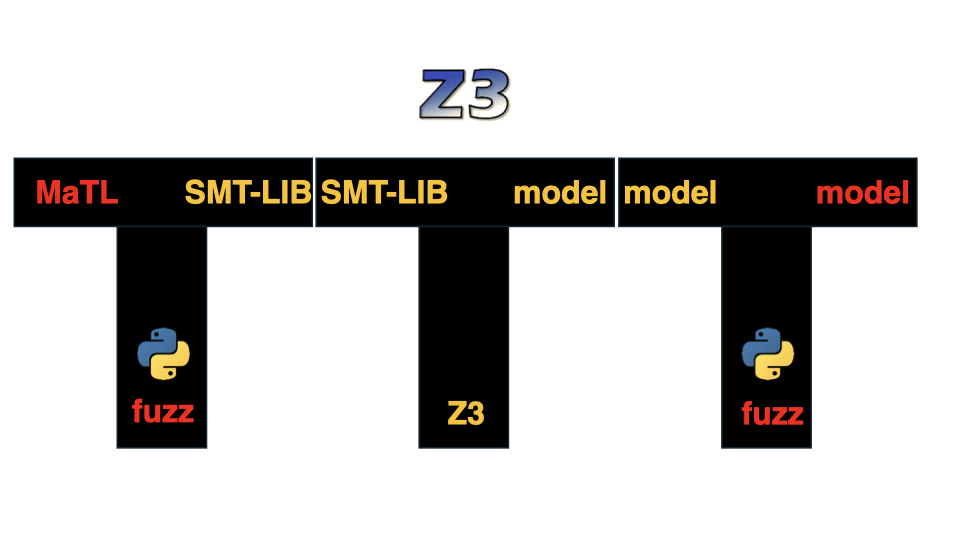
\includegraphics[width=0.8\textwidth]{figures/t-diagram.png}
%\caption{Your caption}
\end{figure}

\begin{block}{}\scriptsize
Our main tasks: 

\begin{enumerate}

\item Design the MaTL temporal logic.
\item Develop translator from MaTL to SMT-LIB. 
\item Refine (further randomize) model generated by Z3.

\end{enumerate}

\end{block}

\end{frame}
  